%
\section{UI framework}
\label{sec:ui-framework}

For the development of the \texttt{Local System} and the \texttt{Remote Client}, it is necessary to use a \gls{ui} Framework, in order to develop a \gls{ui}, making it more user friendly and interactive.
There are several frameworks that can be used in Linux, such as~\cite{ui-lists}:
%
\begin{item-c}
\item Qt;
\item Sciter;
\item Noesis GUI;
\item wxWidgets;
\item GTK+;
\item and so on.
\end{item-c}

For this project, \texttt{Qt} was chosen due to the following reasons:

\begin{item-c}
\item
\emph{Cross development}: it is possible to `develop graphical user interfaces and cross-platform applications, both desktop and embedded'~\cite{qt-bib}.
The framework operates on different types of software and hardware.
\item 
\emph{Cost}:
this framework is \texttt{cost-friendly}, not only because it has a free license, but also because its software development takes less time to develop due to the integrated environment assisting the developer.
\item 
\emph{Implementation}: it is implemented in C++, which means that it is possible to use many libraries.
The wide choice of modules allow the project to have rich functionality and as a result, the software will have a \gls{gui} similar to a native one.
\end{item-c}

\subsection{Qt}

The Qt framework contains a comprehensive set of highly intuitive and modularized C++ library classes and is loaded with APIs to simplify application development~\cite{qt-site}.

\subsubsection{Signals and slots}

In Qt, there's an alternative to the callback technique, using \texttt{signals and slots}. A \texttt{signal} is emitted when a particular event occurs and a \texttt{slot} is a function that is called in response to a particular signal~\cite{qt-signals-slots}.

\begin{item-c}
\item\emph{Signals}: Are emitted by an object when its internal state has changed in some way that might be interesting to the object's client or owner. Signals are also public access functions and can be emitted from anywhere~\cite{qt-signals-slots}.
\item\emph{Slots}: A slot is called when a signal connected to it is emitted. Slots are normal C++ functions and can be called normally; their only special feature is that signals can be connected to them~\cite{qt-signals-slots}.
\end{item-c}

Compared to callbacks, signals and slots are slightly slower because of the increased flexibility they provide, although the difference for real applications is insignificant~\cite{qt-signals-slots}.

\subsubsection{Usage Example}

In Fig.\ref{fig:qt-usage-example} is an example on how Qt can be used and what it can generate:
%
\begin{figure}[!hbt]
\centering
    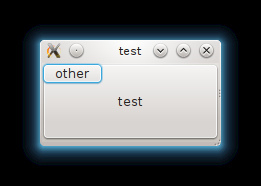
\includegraphics[width=0.3\textwidth]{./img/qt-usage-example.png}
  \caption{Usage example of Qt(withdrawn from~\cite{qt-usage})}%
\label{fig:qt-usage-example}
\end{figure}

The code that generates this \gls{ui} is the following:
%
\lstinputlisting[language=C++, firstline=1,
caption={Implementing a simple window in Qt},
label=lst:qt-usage-ex,
style= custom-cpp]{./listing/qt-usage-ex.cpp}
%

\subsubsection{Configuration with buildroot}
The configuration of Qt in buildroot to run on Raspberry Pi is pretty simple. 
In the $menuconfig$, it is just needed to select \texttt{Target packages}, then select \texttt{Graphic libraries and applications (graphic/text)} and finally select \texttt{Qt5}.

Then on the Qt5 menu select the following options presented on Fig.~\ref{fig:qt-buildroot}.
%
\begin{figure}[!hbt]
\centering
    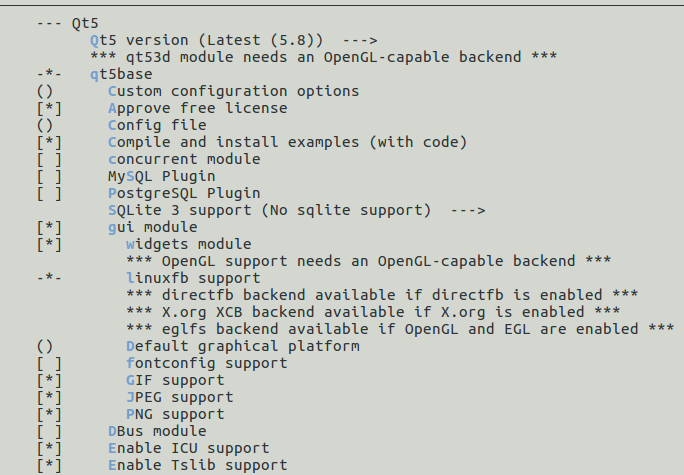
\includegraphics[width=0.6\textwidth]{./img/qt-buildroot.png}
  \caption{Selection of qt package in buildroot(withdrawn from~\cite{qt-root})}%
\label{fig:qt-buildroot}
\end{figure}

In conclusion, \texttt{Qt} is a great option to use on the project due to its features and also because it is very simple to use it on the project's board (Raspberry Pi).
%%% Local Variables:
%%% mode: latex
%%% TeX-master: "../../../dissertation"
%%% End:
